\chapter{Elasticity}

\section{Aim}
To determine the relationship between the extension of elastic material and the load applied

\section{Background Information}
If you stretch a piece of rubber and then release it, it will return to its original shape. If you compress and release a coil spring it will resume its original length and shape. When an object stretches or compresses we say it is deformed because it is not in its original shape. The ability of an object to return to its original shape after deformation is called elasticity. This property is very important for engineers to consider when building machines, tools, and buildings. Also, physicists often find the relationship of elasticity a simple model for many different phenomenon including molecular bonding and different types of oscillatory motion. Therefore, it is necessary to investigate the relationship between the extension of an elastic object and the force applied to it.

\section{Materials}
2 retort stands, spiral spring, pointer, scale pan, masses of (50g, 100g, 150g, 200g, and 250g), meter rule

\section{Procedure}
\begin{enumerate}
\item Hang a spiral spring from a retort stand and attach a scale pan to the other end of the spring.
\item Clamp a meter rule to a second retort stand with the zero mark at the top.
\item	Fix a pointer as shown in the figure.
\item Read and record the pointer position when there is no mass on the scale pan, call it $L_0$.
\item Put a mass of 50g on the scale pan, then read and record the new reading on the meter rule, call it $L$.
\item Repeat procedure (5) with masses of 100g, 150g, 200g, and 250g and tabulate your result including mass and length.
\item Remove the masses from the scale pan and observe.
\end{enumerate}

\begin{figure}[h!]
\centering
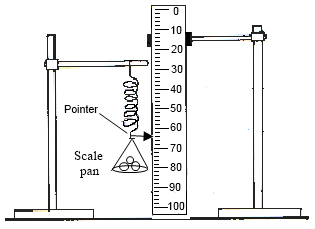
\includegraphics[width=10cm]{./img/elasticity-1.png}
\caption{Elasticity practical setup}
\label{fig:elasticity-1}
\end{figure}

\section{Analysis and Interpretation}
\begin{enumerate}
\item What did you observe when the mass was removed from the spiral spring?
\item Compute the weight and extension $(L-L_0)$ for each mass.
\item Plot a graph of weight (load) against extension.
\item From the graph find the slope of the best fit line.
\end{enumerate}

\section{Conclusion}
From the results of the experiment what is the relationship between the weight (load) and the extension of an elastic material?

\section{Questions for Discussion}
\begin{enumerate}
\item What would happen if you hung a very large mass on the spiral spring?
\item Why can’t we use cotton thread or wire instead of a spiral spring in this experiment?
\item What if we had placed the pointer at the top of the spring, would the experiment still work, why or why not?
\item What is the physical meaning of the slope? Explain it in your own words.
\end{enumerate}

\section{Reflection and Self Assessment}
\begin{enumerate}
\item Did you encounter any problems during the experiment? If yes, what were those problems?
\item What are some applications of elastic materials in your daily life?
\end{enumerate}